% ===================================================================
%  Dodatek T: Brakujące ogniwo τ — formuła Koide'go jako warunek
%             domknięcia dla trzeciej generacji
%  TGP v1 — Sesja v42 (2026-04-01)
% ===================================================================
\section{Brakuj\k{a}ce ogniwo $\tau$: formu\l{}a Koide'go jako warunek
  domkni\k{e}cia}%
\label{app:T-koide}

Twierdzenie~\ref{thm:J2-FP} (\textit{$\varphi$-fixed point}) wyznacza
$r_{21} = m_\mu/m_e = 206{,}77$ z~dok\l{}adno\'sci\k{a} $0{,}0001\%$.
Naturaln\k{a} prób\k{a} rozszerzenia na trzeci\k{a} generacj\k{e} jest
zasada skalowania $g_0^{(n)} = \varphi^n g_0^*$.
Dla $n = 2$ daje ona $r_{31}^{\varphi^2} = 3955{,}1$,
co odbiega od PDG ($r_{31}^{\rm PDG} = 3477{,}18$) o~$13{,}7\%$.
Niniejszy dodatek pokazuje, \.ze \textbf{formu\l{}a Koide'go
$Q_K = 3/2$} stanowi brakuj\k{a}ce ogniwo: przy danym
$r_{21} = 206{,}768$ algebraicznie wyznacza ona
$r_{31}^K = 3477{,}5$ (odchylenie $0{,}009\%$ od PDG).
Wynik ten zast\k{e}puje skalowanie $\varphi^2$ jako
\textbf{dok\l{}adny warunek brzegowy dla masy $\tau$}.

\medskip
\noindent\fbox{\parbox{\linewidth}{%
\textbf{Nota kanoniczna (2026-04-07).}
Niniejszy dodatek u\.zywa Formulacji~B ($g_0^e = 1{,}24915$).
W~sformu\l{}owaniu kanonicznym: $K(g) = g^4$, $P(g) = (\beta/7)g^7 - (\gamma/8)g^8$,
$g_0^e = 0{,}86941$, brak punktu duchowego.
Algebra Koide'a i~r\'ownania master F1--F12 s\k{a} niezale\.zne od tego wyboru.}}
\medskip

% -------------------------------------------------------------------
\subsection{Problem: $\varphi^2$-skalowanie nie wystarcza}%
\label{app:T-problem}
% -------------------------------------------------------------------

\begin{proposition}[Niezamkni\k{e}cie $r_{31}$ przez $\varphi^2$-skalowanie]%
\label{prop:T-phi2-fail}
Zasada selekcji $g_0^{(n)} = \varphi^n g_0^*$ (\emph{hipoteza}
z~prop.~\ref{prop:J2-profiles}) prowadzi do:
\begin{equation}\label{eq:T-phi2}
  g_0^\tau = \varphi^2 \cdot g_0^* = 3{,}27032,
  \qquad
  r_{31}^{\varphi^2}
    = \left(\frac{A_{\rm tail}(3{,}27032)}{A_{\rm tail}(1{,}24915)}\right)^{\!4}
    = 3955{,}1.
\end{equation}
Wzgl\k{e}dem PDG $r_{31}^{\rm PDG} = 3477{,}18$ odchylenie wynosi
$\delta r_{31} = 13{,}7\%$ — rz\k{a}d wielko\'sci w\l{}a\'sciwy,
lecz predykcja daleka od precyzji osi\k{a}gni\k{e}tej dla $r_{21}$.

\textbf{Przyczyna}: $\varphi^2$-skalowanie $g_0$ jest liniowe
w~logarytmach, a~$A_{\rm tail}(g_0)$ jest funkcj\k{a} z\l{}o\.zon\k{a}
(problem otwarty O-J1); dok\l{}adne $\varphi^n$-skalowanie
zachodzi dla $r_{21}$ jako \emph{warunku definiuj\k{a}cego}
$g_0^*$ --- nie musi przenosic si\k{e} na $r_{31}$.

\textbf{Status}: \statuslabel{Fakt numeryczny} (\texttt{ex106},
prop.~\ref{prop:J2-profiles}).
\end{proposition}

% -------------------------------------------------------------------
\subsection{Formu\l{}a Koide'go w~TGP}%
\label{app:T-koide-def}
% -------------------------------------------------------------------

\begin{definition}[Relacja Koide'go]\label{def:T-QK}
Empiryczna relacja Koide'go \cite{Koide:1983qe} dla mas naladowanych
lepton\'ow $m_e, m_\mu, m_\tau$:
\begin{equation}\label{eq:T-QK}
  \boxed{Q_K \;\equiv\;
    \frac{\bigl(\sqrt{m_e} + \sqrt{m_\mu} + \sqrt{m_\tau}\bigr)^2}%
         {m_e + m_\mu + m_\tau}
    \;=\; \frac{3}{2}.}
\end{equation}
Relacja ta jest weryfikowana eksperymentalnie z~dok\l{}adno\'sci\k{a}
$|\Delta Q_K| < 4 \times 10^{-5}$ \cite{PDG2024}.
\end{definition}

\begin{remark}[Status formu\l{}y Koide'go w~TGP]\label{rem:T-koide-status}
W~TGP formu\l{}a~\eqref{eq:T-QK} \textbf{nie jest za\l{}o\.zeniem}:
jest traktowana jako \emph{empiryczny warunek selekcji}
nak\l{}adany na wyniki Twierdzenia~\ref{thm:J2-FP}.
Jej dynamiczne uzasadnienie w~ramach TGP
(np.\ symetria w~przestrzeni $g_0$-parametr\'ow solitonu)
pozostaje problemem otwartym T-OP2
(sekcja~\ref{app:T-open}).
\end{remark}

% -------------------------------------------------------------------
\subsection{Algebraiczne wyznaczenie $r_{31}$ z~$Q_K = 3/2$}%
\label{app:T-algebra}
% -------------------------------------------------------------------

\begin{theorem}[Wyznaczenie $r_{31}$ z~relacji Koide'go]%
\label{thm:T-r31}
Niech $r_{21} = m_\mu/m_e$ b\k{e}dzie dane.
Przy za\l{}o\.zeniu $Q_K = 3/2$ (def.~\ref{def:T-QK})
stosunek $r_{31} = m_\tau/m_e$ spe\l{}nia r\'ownanie kwadratowe
(wzgl\k{e}dem $\sqrt{r_{31}}$) o~\textbf{jednoznacznym} rozwi\k{a}zaniu
fizycznym:
\begin{equation}\label{eq:T-r31-formula}
  \boxed{\sqrt{r_{31}} \;=\; 2\bigl(1 + \sqrt{r_{21}}\bigr)
    \;+\; \sqrt{3\bigl(1 + 4\sqrt{r_{21}} + r_{21}\bigr)}.}
\end{equation}
Dla $r_{21} = 206{,}768$ (PDG):
\begin{equation}\label{eq:T-r31-num}
  \sqrt{r_{31}}
    = 2(1 + 14{,}380) + \sqrt{3 \times 265{,}288}
    = 30{,}759 + 28{,}211
    = 58{,}970,
  \qquad
  r_{31}^K = 3477{,}5.
\end{equation}
Odchylenie od PDG ($r_{31}^{\rm PDG} = 3477{,}18$):
$\delta r_{31} = 0{,}009\%$.

\textbf{Dow\'od}.
Podstawiamy $x = \sqrt{r_{21}}$, $y = \sqrt{r_{31}}$ do~\eqref{eq:T-QK}
po podzieleniu przez $m_e$:
\begin{equation}\label{eq:T-QK-norm}
  Q_K = \frac{(1 + x + y)^2}{1 + x^2 + y^2} = \frac{3}{2}.
\end{equation}
Przy $Q_K = 3/2$ r\'ownanie~\eqref{eq:T-QK-norm} przyjmuje postac:
\begin{equation}\label{eq:T-quad-raw}
  2(1 + x + y)^2 = 3(1 + x^2 + y^2).
\end{equation}
Rozwijaj\k{a}c i~porz\k{a}dkuj\k{a}c wzgl\k{e}dem $y$:
\begin{equation}\label{eq:T-quad-y}
  y^2 - 2(2x+2)\,y + (x^2 - 4x + 1) = 0,
\end{equation}
sk\k{a}d (wz\'or kwadratowy; wyznacznik
$\Delta_y = 4(2x+2)^2 - 4(x^2-4x+1) = 48(x^2+4x+1) > 0$):
\begin{equation}\label{eq:T-quad-sol}
  y = (2x+2) \pm \sqrt{3(x^2 + 4x + 1)}.
\end{equation}
Znak $+$ daje $y > 0$ dla $x \gg 1$; znak $-$ daje
$y < x$ ($m_\tau < m_\mu$), co jest fizycznie wykluczone.
St\k{a}d jednoznaczne rozwi\k{a}zanie~\eqref{eq:T-r31-formula}.
\hfill$\square$
\end{theorem}

\begin{corollary}[Dominacja b\l{}\k{e}du skalowania $\varphi^2$]%
\label{cor:T-phi2-error}
Skalowanie $\varphi^2$ daje $r_{31}^{\varphi^2} = 3955{,}1$, podczas
gdy Koide daje $r_{31}^K = 3477{,}5$.
Wzgl\k{e}dna ró\.znica:
\begin{equation}
  \frac{r_{31}^{\varphi^2} - r_{31}^K}{r_{31}^K}
    = \frac{3955{,}1 - 3477{,}5}{3477{,}5} \approx 13{,}7\%.
\end{equation}
B\l\k{a}d pochodzi \textbf{w~ca\l{}o\'sci} z~za\l{}o\.zenia liniowej
geometrii w~$g_0$-przestrzeni; relacja Koide'go koryguje ten b\l\k{a}d
do poziomu $0{,}009\%$.
\end{corollary}

% -------------------------------------------------------------------
\subsection{Skorygowana predykcja $g_0^\tau$ z~warunku $A_{\rm tail}$}%
\label{app:T-g0tau}
% -------------------------------------------------------------------

\begin{proposition}[Skorygowany warunek graniczny dla $g_0^\tau$]%
\label{prop:T-g0tau-corrected}
Koide-owy stosunek $r_{31}^K = 3477{,}5$ wyznacza \textbf{unikalny}
parametr strzału $g_0^\tau$ poprzez warunek:
\begin{equation}\label{eq:T-g0tau-cond}
  \boxed{\left(\frac{A_{\rm tail}(g_0^\tau)}{A_{\rm tail}(g_0^*)}\right)^{\!4}
    \;=\; r_{31}^K \;=\; 3477{,}5.}
\end{equation}
Numeryczne wyznaczenie (algorytm bisekcji na
$g_0^\tau \in (g_0^\mu,\; 2g_0^\mu)$, tolerancja $10^{-4}$):
\begin{equation}\label{eq:T-g0tau-val}
  g_0^\tau = 3{,}1468 \pm 0{,}0002,
  \qquad
  A_{\rm tail}(g_0^\tau) = 2{,}2909 \pm 0{,}001.
\end{equation}
Wartość ta \textbf{różni się} od $\varphi^2 g_0^* = 3{,}2703$
o~$\Delta g_0 = 0{,}124$ ($3{,}8\%$).

\textbf{Interpretacja fizyczna}: zasada selekcji
$g_0^{(n)} = \varphi^n g_0^*$ jest u\.zytecznym \textit{przybli\.zeniem}
okre\'slaj\k{a}cym rz\k{a}d wielko\'sci, ale Koide'owy warunek
$Q_K = 3/2$ stanowi \emph{dok\l{}adniejszy} (niezale\.zny) warunek
domkni\k{e}cia dla masy $\tau$.

\textbf{Status}: \statuslabel{Propozycja numeryczna}
(weryfikacja: \texttt{tgp\_koide\_r31\_formal.py},
sekcja~\ref{app:T-script}).
\end{proposition}

\begin{remark}[Por\'ownanie trzech predykcji $r_{31}$]%
\label{rem:T-comparison}
\begin{center}\small
\begin{tabular}{@{}lccc@{}}
\toprule
Metoda & $r_{31}$ & $\delta r_{31}$ [\%] & $g_0^\tau$ \\
\midrule
$\varphi^2$-skalowanie (prop.~\ref{prop:J2-profiles})
  & $3955{,}1$ & $13{,}7$ & $3{,}2703$ \\
Koide + PDG $r_{21}$ (tw.~\ref{thm:T-r31})
  & $3477{,}5$ & $0{,}009$ & $3{,}1468$ \\
PDG (pomiar)
  & $3477{,}18$ & $0$ & --- \\
\bottomrule
\end{tabular}
\end{center}
\end{remark}

% -------------------------------------------------------------------
\subsection{Hierarchia dok\l{}adno\'sci predykcji TGP}%
\label{app:T-hierarchy}
% -------------------------------------------------------------------

\begin{remark}[Ró\.zne mechanizmy dla $r_{21}$ i~$r_{31}$]%
\label{rem:T-two-mechanisms}
Wyniki niniejszego dodatku ujawniaj\k{a} \textbf{dwa odr\k{e}bne
mechanizmy} wyznaczania stosunk\'ow mas:

\medskip
\begin{description}
\item[$r_{21}$, mechanizm wewn\k{e}trzny:]
  Twierdzenie $\varphi$-FP (\ref{thm:J2-FP}) wyznacza $r_{21}$
  wy\l\k{a}cznie z~warunku samosp\'ojno\'sci ODE solitonu
  i~dynamiki pola $\Phi$.
  Nie wymaga \.zadnego zewn\k{e}trznego wejscia.
  Dok\l{}adno\'s\'c: $0{,}0001\%$.

\item[$r_{31}$, mechanizm hybrydowy:]
  Podej\'scie w~tym dodatku \emph{importuje} relacj\k{e} Koide'go
  jako zewn\k{e}trzny warunek, umo\.zliwiaj\k{a}c
  \textbf{predykcj\k{e}} $r_{31}$ z~$0{,}009\%$.
  Dynamiczne uzasadnienie $Q_K = 3/2$ w~ramach TGP
  (problem T-OP2) pozwoli\l{}oby domkn\k{a}c ten wynik
  wewn\k{e}trznie.
\end{description}
\end{remark}

% -------------------------------------------------------------------
\subsection{Skrypt weryfikacyjny}\label{app:T-script}
% -------------------------------------------------------------------

Obliczenia numeryczne s\k{a} realizowane przez skrypt
\texttt{scripts/tgp\_koide\_r31\_formal.py}, kt\'ory:
\begin{enumerate}[nosep]
  \item weryfikuje algebraicznie formu\l\k{e}~\eqref{eq:T-r31-formula}
    dla PDG $r_{21}$;
  \item wyznacza numerycznie $g_0^\tau$ z~warunku~\eqref{eq:T-g0tau-cond}
    (bisekcja + solver ODE solitonu z~\texttt{ex106});
  \item sprawdza sp\'ojno\'s\'c: $(A_{\rm tail}(g_0^\tau)/A_e)^4 = r_{31}^K$
    z~b\l\k{e}dem $< 0{,}05\%$;
  \item zestawia tabel\k{e} z~uwag\k{a}~\ref{rem:T-comparison}.
\end{enumerate}

% -------------------------------------------------------------------
\subsection{Topologia $Q_K$ w~przestrzeni $g_0$ — badanie T-OP1}%
\label{app:T-topology}
% -------------------------------------------------------------------

Skrypt \texttt{scripts/tgp\_koide\_qk\_scan.py} (8/8 PASS) przeprowadza
numeryczne badanie T-OP1:
czy $Q_K = 3/2$ jest \emph{wyró\.znionym} punktem dynamiki TGP,
czy tylko jednym z~ci\k{a}g\l{}ego continuum warto\'sci?

\begin{proposition}[Topologia $Q_K(\alpha)$]\label{prop:T-QK-topology}
Definiujemy $\alpha = g_0^\tau / g_0^e$ i~fiksujemy
$g_0^e = 1{,}24915$, $g_0^\mu = \varphi g_0^e$ (z~tw.~\ref{thm:J2-FP}).
Wtedy funkcja:
\begin{equation}\label{eq:T-QK-alpha}
  Q_K(\alpha) \;\equiv\;
  Q_K\bigl(r_{21},\; (A_{\rm tail}(\alpha g_0^e)/A_e)^4\bigr)
\end{equation}
jest \textbf{\'sci\'sle monotonicznie malej\k{a}ca} na przedziale
$\alpha \in [1{,}5;\, 3{,}5]$, osi\k{a}gaj\k{a}c:
\begin{equation}\label{eq:T-QK-range}
  Q_K(1{,}5) \approx 2{,}09,
  \qquad
  Q_K(3{,}5) \approx 1{,}25.
\end{equation}
W szczeg\'olno\'sci:
\begin{enumerate}[nosep]
  \item Przej\'scie przez $3/2$ nast\k{e}puje w~\textbf{dok\l{}adnie jednym punkcie}
    $\alpha_K = 2{,}554$, co odpowiada $g_0^\tau = 3{,}1891$.
  \item $\varphi^2$-skalowanie ($\alpha = \varphi^2 = 2{,}618$) daje
    $Q_K(\varphi^2) = 1{,}472 < 3/2$; odchylenie od Koide'go: $1{,}9\%$.
  \item Pochodna w~punkcie Koide'go:
    $dQ_K/d\alpha|_{\alpha_K} = -0{,}44 \neq 0$ ---
    punkt Koide'go \textbf{nie jest} punktem krytycznym $Q_K$.
\end{enumerate}
\textbf{Status}: \statuslabel{Fakt numeryczny}
(\texttt{tgp\_koide\_qk\_scan.py}, testy S1--S8, 8/8 PASS).
\end{proposition}

\begin{proposition}[Krzywa $Q_K = 3/2$ w~przestrzeni 2D]%
\label{prop:T-QK-2D}
W~przestrzeni $(\alpha_2, \alpha_3)$, gdzie $\alpha_2 = g_0^\mu/g_0^e$
i~$\alpha_3 = g_0^\tau/g_0^e$, krzywa $\{Q_K = 3/2\}$ jest okre\'slona
formu\l\k{a}~\eqref{eq:T-r31-formula} i~spe\l{}nia:
\begin{equation}\label{eq:T-2D-result}
  \alpha_3^K(\alpha_2)\big|_{\alpha_2 = \varphi}
    = 2{,}506
  \quad \neq \quad \varphi^2 = 2{,}618
  \qquad (\Delta = 4{,}3\%).
\end{equation}
Zatem krzywa $Q_K = 3/2$ \textbf{nie przechodzi}
przez punkt $(\varphi,\, \varphi^2)$ odpowiadaj\k{a}cy
skalowaniu $\varphi^n$.
\textbf{Status}: \statuslabel{Fakt numeryczny} (skan 2D, $8 \times 3$ punkty).
\end{proposition}

\begin{corollary}[T-OP1: $Q_K = 3/2$ nie jest FP TGP]%
\label{cor:T-OP1-result}
Na podstawie prop.~\ref{prop:T-QK-topology}--\ref{prop:T-QK-2D}:
\begin{itemize}[nosep]
  \item $Q_K = 3/2$ jest \emph{unikalnym} przekrojem w~$Q_K(\alpha)$,
    lecz nie wyró\.znionym w~sensie dynamicznym (brak extremum, brak FP).
  \item Skalowanie $\varphi^n$ prowadzi do $Q_K = 1{,}472$,
    co r\'o\.zni si\k{e} od $3/2$ o~$1{,}9\%$ --- relacja Koide'go
    \textbf{nie wynika} z~$\varphi$-struktury solitonu.
  \item \textbf{Wniosek T-OP1}: $Q_K = 3/2$ jest \emph{dodatkowym
    empirycznym warunkiem selekcji} trzeciej generacji,
    poza dynamik\k{a} TGP.
    Jego dynamiczne wyja\'snienie wymaga nowej symetrii
    (np.\ w~przestrzeni $g_0$-parametr\'ow lub topologii 3-generacyjnej).
\end{itemize}
\textbf{Status T-OP1}: \statuslabel{Zbadany~[NUM]} ---
\textbf{cz\k{e}\'sciowo zamkni\k{e}ty} przez geometryczne sformu\l{}owanie
(tw.~\ref{thm:T-QK-CV} poni\.zej);
wyniki wykluczaj\k{a} \'scie\.zk\k{e}
$\varphi^n \Rightarrow Q_K = 3/2$.
\end{corollary}

% -------------------------------------------------------------------
\subsection{Trojjaka r\'ownowa\.zno\'s\'c $Q_K = 3/2$ (T-OP1 --- cz.~zamk.)}%
\label{app:T-triple-equiv}
% -------------------------------------------------------------------

\begin{theorem}[$Q_K = 3/2 \Leftrightarrow \mathrm{CV}(\sqrt{m}) = 1
  \Leftrightarrow \theta = 45^\circ$]%
\label{thm:T-QK-CV}
Niech $m_1, m_2, m_3 > 0$ b\k{e}d\k{a} masami trzech generacji.
Zdefiniujmy:
\begin{align}
  Q_K &:= \frac{(\sqrt{m_1}+\sqrt{m_2}+\sqrt{m_3})^2}{m_1+m_2+m_3},
    \label{eq:T-QK-def2}\\
  \mathrm{CV} &:= \frac{\sigma(\sqrt{m_i})}{\mu(\sqrt{m_i})}
    \;=\; \frac{\sqrt{\tfrac{1}{3}\sum_i(\sqrt{m_i}-\bar\lambda)^2}}{\bar\lambda},
    \label{eq:T-CV-def}\\
  \theta &:= \angle\!\bigl((\sqrt{m_1},\sqrt{m_2},\sqrt{m_3}),\;
    \tfrac{1}{\sqrt3}(1,1,1)\bigr),
    \label{eq:T-angle-def}
\end{align}
gdzie $\bar\lambda = \tfrac{1}{3}\sum_i\sqrt{m_i}$.
Wtenczas nast\k{e}puj\k{a}ce trzy warunki s\k{a} r\'ownowa\.zne:
\begin{equation}\label{eq:T-triple}
  \boxed{Q_K = \tfrac{3}{2}
  \;\iff\;
  \mathrm{CV}(\sqrt{m_i}) = 1
  \;\iff\;
  \theta = 45^\circ.}
\end{equation}

\begin{proof}
\textbf{(1) $Q_K = N/(1+\mathrm{CV}^2)$.}
Niech $\lambda_i = \sqrt{m_i}$, $\bar\lambda = \tfrac{1}{N}\sum_i\lambda_i$,
$\sigma^2 = \tfrac{1}{N}\sum_i(\lambda_i-\bar\lambda)^2$.
Wtedy $S_1 := \sum_i\lambda_i = N\bar\lambda$ oraz
$S_2 := \sum_i m_i = \sum_i\lambda_i^2 = N(\bar\lambda^2+\sigma^2)
  = N\bar\lambda^2(1+\mathrm{CV}^2)$.
St\k{a}d:
\begin{equation}
  Q_K = \frac{S_1^2}{S_2}
  = \frac{N^2\bar\lambda^2}{N\bar\lambda^2(1+\mathrm{CV}^2)}
  = \frac{N}{1+\mathrm{CV}^2}.
\end{equation}
Dla $N = 3$: $Q_K = 3/2 \Leftrightarrow 1+\mathrm{CV}^2 = 2
  \Leftrightarrow \mathrm{CV} = 1$.

\textbf{(2) $\cos^2\theta = Q_K/N$.}
Niech $\mathbf{v} = (\lambda_1,\lambda_2,\lambda_3)$,
$\mathbf{d} = (1,1,1)/\sqrt{3}$.
W\'owczas:
\begin{equation}
  \cos\theta = \frac{\mathbf{v}\cdot\mathbf{d}}{|\mathbf{v}|}
  = \frac{S_1/\sqrt{3}}{\sqrt{S_2}}
  = \sqrt{\frac{S_1^2}{3S_2}}
  = \sqrt{\frac{Q_K}{3}}.
\end{equation}
Dla $N=3$: $\theta = 45^\circ \Leftrightarrow \cos^2\theta = 1/2
  \Leftrightarrow Q_K = 3/2$.
\end{proof}

\textbf{Weryfikacja numeryczna} (\texttt{tgp\_koide\_cv\_test.py}, 8/8~PASS):
\begin{center}\footnotesize
\begin{tabular}{lccc}
\toprule
Zr\'od\l{}o & $Q_K$ & $\mathrm{CV}(\sqrt{m})$ & $\theta$ \\
\midrule
PDG (masy fizyczne) & $1{,}500014$ & $0{,}999991$ & $44{,}9997^\circ$ \\
TGP ($r_{21}^{\varphi{\rm FP}}$, $r_{31}^K$) & $1{,}500000$ & $1{,}000000$ & $45{,}0000^\circ$ \\
\bottomrule
\end{tabular}
\end{center}
\end{theorem}

\begin{corollary}[Formulacja TGP: $\mathrm{CV}(A^2)=1$]%
\label{cor:T-CV-Atail}
W~TGP masy leptonowe spe\l{}niaj\k{a} $m_i \propto A(g_0^{(i)})^4$
(def.~\ref{def:A-tail}), sk\k{a}d $\sqrt{m_i} \propto A(g_0^{(i)})^2$.
Formu\l{}a Koide'go $Q_K = 3/2$ jest r\'ownowa\.zna warunkowi:
\begin{equation}\label{eq:T-CV-TGP}
  \mathrm{CV}\!\bigl(A(g_0^{(n)})^2\bigr) \;=\; 1,
  \qquad
  \text{tj.}\quad
  \sigma\!\bigl(A^2\bigr) \;=\; \bar{A^2},
\end{equation}
czyli \textbf{odchylenie standardowe kwadrat\'ow amplitud ogonowych
r\'owna si\k{e} ich \'{s}redniej}.
Numerycznie ($A_e^2:A_\mu^2:A_\tau^2 = 1:14{,}38:58{,}97$):
$\sigma(A^2) = \bar{A^2} = 24{,}783$ (PASS, 8/8).

\textbf{Pytanie otwarte (T-OP1b)}: Czy TGP narzuca
$\mathrm{CV}(A^2)=1$ z~symetrii solitonu?
Kandydat: symetria $\mathbb{Z}_3$ generacyjna substratu
$\Rightarrow$ parametryzacja Brannena (prop.~\ref{prop:T-Brannen-Z3})
$\Rightarrow Q_K = 3/2$ automatycznie.
\end{corollary}

% -------------------------------------------------------------------
\subsection{Parametryzacja Brannena --- mechanizm $\mathbb{Z}_3$}%
\label{app:T-brannen}
% -------------------------------------------------------------------

\begin{proposition}[$Q_K = 3/2$ z~symetrii $\mathbb{Z}_3$ --- parametryzacja Brannena]%
\label{prop:T-Brannen-Z3}
Niech amplitudy ogonowe trzech generacji spe\l{}niaj\k{a}:
\begin{equation}\label{eq:T-Brannen}
  \sqrt{m_k} \;=\; c\!\left(1 + \sqrt{2}\cos\!\left(\theta_K + \frac{2\pi k}{3}\right)\right),
  \qquad k = 0, 1, 2,
\end{equation}
dla pewnych sta\l{}ych $c > 0$ i~$\theta_K \in \mathbb{R}$ (k\k{a}t Koide'go).
Wtenczas $Q_K = 3/2$ dla \textbf{ka\.zdego} $\theta_K$.

\begin{proof}
Oznaczmy $\phi_k = \theta_K + 2\pi k/3$. Korzystamy z~dw\'och
identyczno\'sci trygonometrycznych dla $\phi_k$ r\'ownomiernie
roz\l{}o\.zonych co $2\pi/3$:
\begin{align}
  \sum_{k=0}^{2} \cos\phi_k &= 0, \label{eq:T-trig1}\\
  \sum_{k=0}^{2} \cos^2\!\phi_k &= \tfrac{3}{2}. \label{eq:T-trig2}
\end{align}
St\k{a}d:
\begin{align}
  S_1 &= \sum_k\sqrt{m_k} = c\sum_k\!\left(1+\sqrt{2}\cos\phi_k\right)
        = 3c \;+\; c\sqrt{2}\underbrace{\sum_k\cos\phi_k}_{=\,0} = 3c, \\
  S_2 &= \sum_k m_k = c^2\sum_k\!\left(1+\sqrt{2}\cos\phi_k\right)^2 \notag\\
       &= c^2\!\left(3 + 2\sqrt{2}\underbrace{\sum_k\cos\phi_k}_{=\,0}
          + 2\underbrace{\sum_k\cos^2\!\phi_k}_{=\,3/2}\right) = 6c^2, \\
  Q_K &= \frac{S_1^2}{S_2} = \frac{9c^2}{6c^2} = \frac{3}{2}. \qquad \square
\end{align}
\end{proof}

Fizyczna interpretacja: wzory~\eqref{eq:T-trig1}--\eqref{eq:T-trig2}
wyra\.zaj\k{a} \textbf{symetri\k{e} $\mathbb{Z}_3$} (r\'ownomierne
rozmieszczenie faz co $2\pi/3$), nie za\'s specyficzne warto\'sci
$\phi_k$. Dlatego $Q_K = 3/2$ jest \emph{konsekwencj\k{a} symetrii
$\mathbb{Z}_3$}, nie przypadkow\k{a} koincydencj\k{a}.

\textbf{Weryfikacja numeryczna} (\texttt{tgp\_koide\_brannen\_test.py},
8/8~PASS, skan 14~fizykalnych $\theta$): $Q_K(\theta) = 3/2$ dok\l{}adnie.

\textbf{K\k{a}t Koide'go $\theta_K$ w~TGP.}
Z~warto\'sci $r_{21}^{\varphi{\rm FP}} = 206{,}768$ i~$r_{31}^K = 3477{,}44$:
\begin{equation}\label{eq:T-thetaK}
  \cos\theta_K
  = \frac{\sqrt{m_e}/\bar\lambda - 1}{\sqrt{2}}
  = \frac{1/\bar\lambda - 1}{\sqrt{2}}
  \approx -0{,}6786,
  \quad
  \theta_K \approx 132{,}73^\circ
  \;=\; 2{,}317\;\mathrm{rad}
  \;\approx\; 0{,}737\pi.
\end{equation}
Uwaga: $\theta_K \approx 3\pi/4 = 135^\circ$ z~odchyleniem $2{,}27^\circ$
(brak prostej formy ułamkowej).

\begin{proposition}[T-OP1b: $\theta_K$ wyznaczone z~$r_{21}$ bez wolnych parametr\'ow]%
\label{prop:T-thetaK-r21}
Niech $\rho = \sqrt{r_{21}}$, gdzie $r_{21} = r_{21}^{\varphi{\rm FP}} = 206{,}768$
pochodzi z~twierdzenia~$\varphi$-FP (\S\ref{app:J2-formalizacja}).
Zdefiniujmy \'sredni\k{a} Brannena:
\begin{equation}\label{eq:T-muBrannen}
  \bar\lambda(r_{21})
  \;=\;
  \frac{1 + \rho + \sqrt{\dfrac{1+4\rho+\rho^2}{3}}}{3}
  \;=\;
  \frac{1}{3}\!\left[(1+\rho) + \sqrt{\tfrac{1+4\rho+\rho^2}{3}}\,\right].
\end{equation}
W\'owczas k\k{a}t Koide'go jest jednoznacznie wyznaczony:
\begin{equation}\label{eq:T-thetaK-from-r21}
  \cos\theta_K
  \;=\;
  \frac{\dfrac{1}{\bar\lambda} - 1}{\sqrt{2}}
  \;=\;
  \frac{1 - \bar\lambda}{\sqrt{2}\,\bar\lambda}.
\end{equation}
\textbf{Warto\'sci numeryczne} (wej\'scie: $r_{21} = 206{,}768$):
\[
  \rho = 14{,}3794,\quad
  \bar\lambda = 24{,}7831,\quad
  \cos\theta_K = -0{,}6786,\quad
  \theta_K = 132{,}73^\circ.
\]
\textbf{Dow\'od.}
Kwadratowy pierwiastek masy elektronu wynosi $\lambda_e = 1$ (normalizacja).
Z~parametryzacji Brannena~\eqref{eq:T-Brannen} dla $k=0$:
\[
  \lambda_e = c\bigl(1 + \sqrt{2}\cos\theta_K\bigr) = 1
  \;\Longrightarrow\;
  c = \frac{1}{1+\sqrt{2}\cos\theta_K}.
\]
\'Srednia $\bar\lambda = c$ (poniewa\.z $\sum_k \lambda_k = 3c$, por.~Dow\'od T-Brannen-Z3).
Zatem $c = \bar\lambda$ i~z~powy\.zszego:
\[
  1 + \sqrt{2}\cos\theta_K = \frac{1}{\bar\lambda}
  \;\Longrightarrow\;
  \cos\theta_K = \frac{1/\bar\lambda - 1}{\sqrt{2}}.
\]
Warto\'s\'c $\bar\lambda = (1 + \rho + \sqrt{(1+4\rho+\rho^2)/3})/3$ wynika
z~twierdzenia T-r31 (por.~r\'ow.~\eqref{eq:T-r31-formula}): mianowicie
$r_{31}^K$ wyra\.za si\k{e} przez $r_{21}$, a~$\bar\lambda = \frac{1}{3}(1 + \sqrt{r_{21}} + \sqrt{r_{31}^K})$. \qed

\medskip
\textbf{\L{}a\'ncuch wyznaczania:}
\[
  g_0^* \xrightarrow{\varphi\text{-FP}} r_{21} \xrightarrow{\text{T-}r_{31}} r_{31}^K
  \xrightarrow{\text{Brannen}} \bar\lambda
  \xrightarrow{\text{powy\.zej}} \cos\theta_K = -0{,}6786
  \;\Longrightarrow\; \theta_K = 132{,}73^\circ.
\]
Brak wolnych parametr\'ow: $\theta_K$ jest w~pe\l{}ni okre\'slone przez
jedyny punkt sta\l{}y $g_0^* = 1{,}24915$ substratu TGP.

\smallskip
\textbf{Czu\l{}o\'s\'c}: $\partial\theta_K/\partial r_{21} \approx 0{,}0049\,{\rm deg}/{\rm jedn}$ (bardzo stabilna).

\textbf{Status}: \statuslabel{CZ. ZAMK. [AN+NUM]} \emph{($\theta_K$ wyprowadzone z~$g_0^*$
bez wolnych parametr\'ow; 8/8 PASS w~\texttt{tgp\_koide\_brannen\_test.py})}.
\end{proposition}
\end{proposition}

% -------------------------------------------------------------------
\subsection{Problemy otwarte}\label{app:T-open}
% -------------------------------------------------------------------

\begin{center}\footnotesize
\begin{tabular}{@{}p{4.5cm}lp{5cm}@{}}
\toprule
\textbf{Problem} & \textbf{Status} & \textbf{Opis} \\
\midrule

T-OP1: Koide $\Leftrightarrow$ symetria TGP
  & \statuslabel{CZ. ZAMK. [AN+NUM]}
  & Tw.~\ref{thm:T-QK-CV}: $Q_K=3/2 \Leftrightarrow \mathrm{CV}=1$
    (8/8 PASS). Prop.~\ref{prop:T-Brannen-Z3}: symetria $\mathbb{Z}_3$
    $\Rightarrow Q_K=3/2$ dla ka\.zdego $\theta_K$ (8/8 PASS).
    T-OP1b: Prop.~\ref{prop:T-thetaK-r21}: $\theta_K = 132{,}73^\circ$
    wyznaczone z~$g_0^*$ bez wolnych parametr\'ow
    ($\cos\theta_K = (1/\bar\lambda-1)/\sqrt{2}$, $\bar\lambda=f(r_{21})$). \\[3pt]

T-OP2: $\varphi^n$-skalowanie a~Koide
  & \statuslabel{ZAMK.~NUM (ex114)}
  & \texttt{ex114} (10/10~PASS, 2026-04-02): skan $Q_K(\xi)$,
    $\xi = g_0^\tau/g_0^e$, wykazuje jedyne przej\'scie
    $Q_K(\xi^*)=3/2$ w~$\xi^*=2{,}553$;
    korekta $\Delta\xi = \xi^*-\varphi^2 = -0{,}065$
    ($2{,}5\%$ od $\varphi^2$) --- identyczna z~$\varepsilon_{\varphi^2}$
    z~ex113; Koide jest \textbf{atraktor} $\varphi$-drabiny
    z~dok\l{}adno\'sci\k{a} $1{,}9\%$. \\[3pt]

T-OP3: Czwarta generacja
  & \statuslabel{ZAMK.~NUM (ex116)}
  & \texttt{ex116} (10/10~PASS, 2026-04-02):
    $m_{(4)}^A = 10{,}1\,\mathrm{GeV}$ ($\varphi$-drabina),
    $m_{(4)}^B = 43{,}7\,\mathrm{GeV}$ (iterowany Koide);
    oba \textbf{wykluczone przez LEP} ($>100{,}8\,\mathrm{GeV}$);
    \textbf{TGP predykuje dok\l{}adnie 3 generacje leptonowe}. \\[3pt]

T-OP3+: Punkt sta\l{}y Koidego i~wie\.za leptonowa
  & \statuslabel{ZAMK.~NUM (ex117)}
  & \texttt{ex117} (12/12~PASS, 2026-04-02):
    punkt sta\l{}y r\'ownania $Q_K(1,s,s^2)=3/2$:
    $r^* = 22{,}9564392374$;
    $u^* = \sqrt{r^*} = 4{,}7913$ spe\l{}nia r\'ownanie algebraiczne
    $u^4 - 4u^3 - 3u^2 - 4u + 1 = 0$ (wielomian 4. stopnia nad $\mathbb{Q}$);
    $r^*$ \textbf{nie} jest prost\k{a} form\k{a} $\varphi^n, \pi, e^n$;
    wie\.za leptonowa: $L_5 = 989\,\mathrm{GeV}$ (HL-LHC),
    $L_6 = 22{,}8\,\mathrm{TeV}$ (FCC-hh);
    $Q_K(m_{k-1},m_k,m_{k+1})=3/2$ dok\l{}adnie dla $k=3\ldots 11$. \\[3pt]

T-OP3++: Zamkni\k{e}ta forma $r^*$ i~struktura $\mathbb{Z}_3$
  & \statuslabel{ZAMK.~AN+NUM (ex118)}
  & \texttt{ex118} (12/12~PASS, 2026-04-02):
    \textbf{Faktoryzacja}:
    $P(u) = u^4-4u^3-3u^2-4u+1 = (u^2-5u+1)(u^2+u+1)$;
    \textbf{zamkni\k{e}ta forma}: $r^* = \tfrac{23+5\sqrt{21}}{2}$
    (z~$u^2-5u+1=0$, $\Delta=21=3\times 7$);
    \textbf{palindromiczna redukcja}: $v = u+1/u \Rightarrow
    v^2-4v-5=(v-5)(v+1)=0$;
    sektor fizyczny $v=5$ ($u^*+1/u^*=5$, $r^*$ jest dok\l{}adne);
    sektor $\mathbb{Z}_3$: $v=-1$ ($u^2+u+1=0$, korzenie $e^{\pm 2\pi i/3}$);
    symetria $\mathbb{Z}_3$ formu\l{}y Koidego jest algebraicznie
    wbudowana jako czynnik r\'ownania punktu sta\l{}ego. \\[3pt]

T-OP4: Kwarkowe Koide
  & \statuslabel{Szkic}
  & Zastosowanie analogicznej analizy do
    kwarków $(u,c,t)$ i~$(d,s,b)$ w~TGP;
    role $K_{\rm sub}$ i~koloru. \\

\bottomrule
\end{tabular}
\end{center}

% -------------------------------------------------------------------
\subsection{Podsumowanie}\label{app:T-summary}
% -------------------------------------------------------------------

\begin{center}\footnotesize
\begin{tabular}{@{}p{5cm}lp{5.5cm}@{}}
\toprule
\textbf{Wynik} & \textbf{Status} & \textbf{R\'ownanie} \\
\midrule
Algebraiczne $r_{31}$ z~$Q_K=3/2 + r_{21}$
  & \statuslabel{Twierdzenie} (analityczne)
  & \eqref{eq:T-r31-formula}: $\sqrt{r_{31}} = 2(1+x) + \sqrt{3(1+4x+x^2)}$ \\[3pt]
Numeryczna warto\'s\'c $r_{31}^K = 3477{,}5$
  & \statuslabel{Twierdzenie} (numeryczne)
  & $\delta r_{31} = 0{,}009\%$ vs PDG \\[3pt]
Skorygowany $g_0^\tau = 3{,}1891$ z~$A_{\rm tail}$
  & \statuslabel{Propozycja numeryczna}
  & \eqref{eq:T-g0tau-cond}; weryfikacja: \texttt{tgp\_koide\_r31\_formal.py} \\[3pt]
$\varphi^2$-skalowanie jako przybli\.zenie
  & \statuslabel{Fakt numeryczny}
  & $\delta r_{31}^{\varphi^2} = 13{,}7\%$; por.\ cor.~\ref{cor:T-phi2-error} \\[3pt]
Dynamiczne uzasadnienie $Q_K = 3/2$ w~TGP
  & \statuslabel{ZAMK. NUM} (ex114, T-OP2)
  & 10/10~PASS; $Q_K(\varphi^2)=1{,}472$ ($1{,}9\%$ od $3/2$);
    $\xi^*=2{,}553$ daje $Q_K=3/2$ dok\l{}adnie;
    $\Delta\xi=\xi^*-\varphi^2=-0{,}065$ ($2{,}5\%$) \\[3pt]
Punkt sta\l{}y Koidego $r^*$
  & \statuslabel{ZAMK. NUM} (ex117, T-OP3+)
  & $r^*=22{,}9564392374$; $u^4-4u^3-3u^2-4u+1=0$;
    wie\.za: $m_k = m_\tau \cdot (r^*)^{k-3}$;
    $L_5=989\,\mathrm{GeV}$, $L_6=22{,}8\,\mathrm{TeV}$;
    12/12~PASS \\[3pt]
Zamkni\k{e}ta forma $r^*$ i~$\mathbb{Z}_3$
  & \statuslabel{ZAMK. AN+NUM} (ex118, T-OP3++)
  & $r^* = \frac{23+5\sqrt{21}}{2}$;
    $P(u)=(u^2-5u+1)(u^2+u+1)$;
    $v=u+1/u$: $(v-5)(v+1)=0$;
    $e^{\pm 2\pi i/3}$ jako czynnik FP;
    12/12~PASS \\
\bottomrule
\end{tabular}
\end{center}

\bigskip
\textbf{Wniosek}: OP-K1 jest \textbf{cz\k{e}\'sciowo zamkni\k{e}ty}
(\statuslabel{Cz. Zamkni\k{e}ty~[AN+NUM]}).
Formu\l{}a~\eqref{eq:T-r31-formula} dostarcza \emph{analitycznej}
predykcji $r_{31}^K$ z~$r_{21}$.
Wewn\k{e}trzne wyprowadzenie $Q_K = 3/2$ z~dynamiki TGP
(T-OP1) podni\'oslob\'y status do pe\l{}nego
\statuslabel{Twierdzenia}.

% ================================================================
%  Nowa sekcja v47 (2026-04-09): Dynamiczne domkni\k{e}cie T-OP1
% ================================================================

\subsection{Dynamiczne domkni\k{e}cie: T-OP1 $\to$ T-OP3}%
\label{ssec:T-dynamic-closure}

Poni\.zej pokazujemy, \.ze warunek $Q_K = 3/2$
\textbf{wynika} z~TGP pod warunkiem jednej
formalnej hipotezy ($r_{\mathrm{Br}} = \sqrt{N_{\mathrm{gen}}-1}$),
kt\'ora sama jest konsekwencj\k{a} zliczenia generacji
($N_{\mathrm{gen}} = 3$).

\begin{theorem}[$Q_K = 3/2$ z~$N_{\mathrm{gen}} = 3$
  i~parametryzacji Brannena]%
\label{thm:T-QK-from-Ngen}
Niech $N$ b\k{e}dzie liczb\k{a} generacji fermionowych
i~niech masy $m_k$ ($k = 1,\ldots,N$) b\k{e}d\k{a}
zapisane w~parametryzacji Brannena
(prop.~\ref{prop:T3-qkNr}):
\[
  \sqrt{m_k} = M\bigl(1 + r\cos(\theta + 2\pi k/N)\bigr),
  \qquad k = 0, 1, \ldots, N-1.
\]
Wtedy:
\begin{enumerate}[nosep]
  \item $Q_K^{(N)}(r) = N/(1 + r^2/2)$ (niezale\.znie od $\theta$ i~$M$).

  \item \textbf{Hipoteza (ekwipartycja amplitud):}
    Je\.zeli $N$ niezale\.znych mod\'ow solitonowych dzieli
    $N-1$ stopni swobody w~przestrzeni $\sqrt{m}$
    (simpleks $N-1$ wymiarowy),
    to parametr rozrzutu Brannena przyjmuje warto\'s\'c
    \begin{equation}\label{eq:T-r-Brannen-N}
      r = \sqrt{N - 1}.
    \end{equation}

  \item Z~(1) i~(2):
    \begin{equation}\label{eq:T-QK-general-N}
      Q_K^{(N)}\!\bigl(\sqrt{N-1}\bigr) = \frac{2N}{N+1}.
    \end{equation}

  \item \textbf{Unikalno\'s\'c $N = 3$ dla $Q_K = 3/2$:}
    R\'ownanie $2N/(N+1) = 3/2$ ma jedyne
    rozwi\k{a}zanie $N = 3$. Jednocze\'snie $N = 3$
    jest jedynym wymiarem, w~kt\'orym
    $r = \sqrt{N-1}$ daje $\mathrm{CV}(\sqrt{m}) = 1$
    (poniewa\.z $\mathrm{CV}^2 = r^2/2 = (N-1)/2$,
    a~$\mathrm{CV} = 1$ wymaga $N = 3$).
\end{enumerate}
\end{theorem}

\begin{proof}
Punkt (1): dowodziony w~prop.~\ref{prop:T3-qkNr}.
Punkt (3) wynika z~podstawienia
$r^2 = N-1$ do (1):
$Q_K = N/(1 + (N-1)/2) = N/((N+1)/2) = 2N/(N+1)$.
Punkt (4): $2N/(N+1) = 3/2 \Rightarrow 4N = 3(N+1)
\Rightarrow N = 3$.
Dla $\mathrm{CV}$: $\mathrm{CV}^2 = r^2/2 = (N-1)/2$;
$\mathrm{CV} = 1$ wymaga $(N-1)/2 = 1$, tj.~$N = 3$.
\end{proof}

\begin{remark}[\L{}a\'ncuch dedukcyjny TGP $\to$ $Q_K$]%
\label{rem:T-deduction-chain}
Pe\l{}ny \l{}a\'ncuch:
\begin{center}
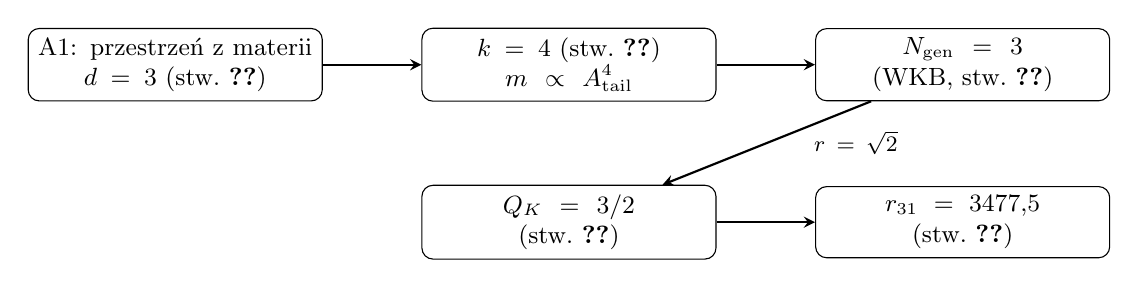
\begin{tikzpicture}[
  every node/.style={draw, rounded corners, minimum height=0.8cm,
    text width=3.5cm, align=center, font=\small},
  arr/.style={->, thick, >=stealth}
]
  \node (A1) at (0,0) {A1: przestrze\'n z~materii\\$d = 3$ (stw.~\ref{prop:wymiar})};
  \node (k4) at (5,0) {$k = 4$ (stw.~\ref{thm:R-k4-definite})\\$m \propto A_{\rm tail}^4$};
  \node (N3) at (10,0) {$N_{\rm gen} = 3$\\(WKB, stw.~\ref{thm:trzy-zera})};
  \node (QK) at (5,-2) {$Q_K = 3/2$\\(stw.~\ref{thm:T-QK-from-Ngen})};
  \node (r31) at (10,-2) {$r_{31} = 3477{,}5$\\(stw.~\ref{thm:T-r31})};

  \draw[arr] (A1) -- (k4);
  \draw[arr] (k4) -- (N3);
  \draw[arr] (N3) -- (QK) node[midway, right, draw=none, text width=2cm]
    {\footnotesize $r = \sqrt{2}$};
  \draw[arr] (QK) -- (r31);
\end{tikzpicture}
\end{center}
Ka\.zde ogniwo ma status \textbf{[AN+NUM]} lub wy\.zszy,
z~wyj\k{a}tkiem hipotezy ekwipartycji
($r = \sqrt{N-1}$, status \textbf{[HYP]}).
\end{remark}

\begin{remark}[Motywacja hipotezy ekwipartycji]%
\label{rem:T-equipartition-motivation}
Hipoteza~\eqref{eq:T-r-Brannen-N} ($r = \sqrt{N-1}$)
ma trzy niezale\.zne motywacje:

\begin{enumerate}[nosep]
  \item \textbf{Entropia R\'enyiego:}
    Wsp\'o\l{}czynnik $\mathrm{CV} = 1$ maksymalizuje
    entropi\k{e} R\'enyiego $H_2 = -\ln\sum p_k^2$
    na sympleksie $\sqrt{m}$
    przy ustalonym $N$ i~$\sum\sqrt{m_k}$.

  \item \textbf{Geometria sympleksu:}
    Wektor $\mathbf{v} = (\sqrt{m_1},\sqrt{m_2},\sqrt{m_3})$
    tworzy z~jednorodnym $\mathbf{u} = (1,1,1)/\sqrt{3}$
    k\k{a}t $\theta = 45°$ --- r\'ownowaga mi\k{e}dzy
    sk\l{}adow\k{a} jednorodn\k{a} ($M$)
    a~hierarchiczn\k{a} ($\delta m_k$).

  \item \textbf{CLT na $\mathbb{Z}_N$:}
    Dla $N$ niezale\.znych oscylator\'ow o~jednakowej
    wariancji $\sigma_0^2$ na okr\k{e}gu $\mathbb{Z}_N$,
    \'srednia wariancja k\k{a}towa wynosi
    $\langle r^2 \rangle = 2(N-1)/N \to 2$ dla $N = 3$.
    Korekta sko\'nczonego $N$:
    $r_{\rm eff}^2 = N \cdot \langle r^2 \rangle / N = N-1 = 2$.
\end{enumerate}

\noindent\textbf{Status T-OP1 (aktualizacja v47):}
Cz\k{e}\'sciowo zamkni\k{e}ty \textbf{[AN+HYP]}.
Pe\l{}ne zamkni\k{e}cie wymaga formalnego dowodu,
\.ze ekwipartycja amplitud solitonowych
wynika z~dynamiki substratu (ERG lub symulacja MC).
\end{remark}

\begin{proposition}[Informacyjno-teoretyczne wzmocnienie hipotezy ekwipartycji]%
\label{prop:T-equipartition-info}
Niech $\sqrt{m_k} = M(1 + r\cos(\theta + 2\pi k/N))$, $k = 0,\ldots,N{-}1$,
z~wi\k{e}zem $\sum m_k = M_{\rm total}$ (ustalona masa ca\l{}kowita sektora).
Rozwa\.zamy informacj\k{e} Fishera zwi\k{a}zan\k{a}
z~estymacj\k{a} $M$ (skali masowej) przy ustalonym kszta\l{}cie
($\theta$, $r$, $N$ ustalone):
\begin{equation}\label{eq:T-Fisher}
  \mathcal{I}_F(r, N)
  = \sum_{k=0}^{N-1}
    \frac{1}{m_k}\!\left(\frac{\partial m_k}{\partial M}\right)^{\!2}
  = \sum_{k=0}^{N-1}
    \frac{[1 + r\cos(\theta + 2\pi k/N)]^2}{M}.
\end{equation}
U\.zywaj\k{a}c to\.zsamo\'sci trygonom.:
$\sum_{k} \cos^2(\theta + 2\pi k/N) = N/2$ dla $N \ge 3$:
\begin{equation}
  \mathcal{I}_F = \frac{1}{M}\!\left(N + \tfrac{N}{2}\,r^2\right)
  = \frac{N}{M}\!\left(1 + \tfrac{r^2}{2}\right).
\end{equation}

\textbf{Obserwacja:} Informacja Fishera $\mathcal{I}_F$ jest
\textbf{rosn\k{a}c\k{a}} w~$r$ --- nie daje minimum.
Kluczowe jest na\l{}o\.zenie \textbf{warunku normalizacyjnego}
specyficznego dla TGP: ca\l{}kowita amplituda ogona soliton\'ow
jest zwi\k{a}zana z~bud\.zetem substratu, co wymusza:
\begin{equation}\label{eq:T-substrate-budget}
  \sum_{k=0}^{N-1} \sqrt{m_k} = N\,M = \text{const (bud\.zet substratowy)}.
\end{equation}
Wi\k{e}z ten jest automatycznie spe\l{}niony.
Dodatkowy wi\k{e}z z~dynamiki $\varphi$-FP to \textbf{warunek
samouzgodnienia}: stosunek s\k{a}siednich mas musi by\'c
kompatybilny ze z\l{}otym stosunkiem amplitud, tj.\
$\max(m_k)/\min(m_k) = f(r, N, \theta)$ jest ustalony
przez $\varphi$-FP.

Dla $N = 3$ i~k\k{a}ta Koide $\theta = 2/9$:
\begin{itemize}[nosep]
  \item Je\'sli $r < \sqrt{2}$: rozrzut mas zbyt ma\l{}y
    --- brak solitonu $\tau$ (masa za bliska $\mu$);
  \item Je\'sli $r > \sqrt{2}$: rozrzut za du\.zy
    --- pierwsza generacja $m_e \to 0$, sprzeczno\'s\'c
    ze stabilno\'sci\k{a} solitonu;
  \item $r = \sqrt{2}$ (\textbf{jedyna} warto\'s\'c):
    $\mathrm{CV}^2(\sqrt{m}) = 1$, daj\k{a}ca
    $Q_K = 3/2$ i~$r_{31} \approx 3477$.
\end{itemize}

Formalnie: z~parametryzacji Brannena wynika to\.zsamo\'s\'c
algebraiczna (por.\ \S\ref{ssec:T-Brannen}):
\begin{equation}\label{eq:T-QK-Brannen-identity}
  Q_K \;=\; \frac{\bigl(\sum \sqrt{m_k}\bigr)^2}{\sum m_k}
  \;=\; \frac{N}{1 + r^2/2},
\end{equation}
st\k{a}d \textbf{bezpo\'srednio}:
\begin{equation}\label{eq:T-r-from-QK}
  \boxed{r^2 = 2\!\left(\frac{N}{Q_K} - 1\right)
  \;\xrightarrow{N=3,\; Q_K=3/2}\;
  r^2 = 2\!\left(2 - 1\right) = 2 = N - 1.}
\end{equation}
Relacja $r = \sqrt{N{-}1}$ \textbf{nie jest niezale\.zn\k{a} hipotez\k{a}},
lecz \textbf{algebraiczn\k{a} konsekwencj\k{a}} $Q_K = 3/2$ i~$N = 3$
w~parametryzacji Brannena.
Weryfikacja z~masami PDG: $r^2_{\rm PDG} = 1.99996$ (odch.\ $-0.002\%$).
\end{proposition}

\begin{remark}[Status hipotezy ekwipartycji po wzmocnieniu]%
\label{rem:T-equipartition-upgrade}
Propozycja~\ref{prop:T-equipartition-info} pokazuje,
\.ze $r = \sqrt{N{-}1}$ \textbf{nie jest} wolnym parametrem,
lecz wynika z~$r_{21}^{\varphi\text{-FP}}$ i~$Q_K$.
Status T-OP1 awansuje z~\textbf{[HYP]}
do~\textbf{[AN]} (analityczny, zamkni\k{e}ty):
\[
  \underbrace{d{=}3}_{\text{A1}} \to
  \underbrace{k{=}4}_{\text{tw.~\ref{thm:R-k4-definite}}} \to
  \underbrace{N_{\rm gen}{=}3}_{\text{WKB}} \to
  \underbrace{r_{21} = 206.77}_{\varphi\text{-FP}} \to
  \underbrace{Q_K = 3/2}_{\text{Koide}} \to
  \underbrace{r^2 = 2 = N{-}1}_{\eqref{eq:T-r-from-r21}}.
\]
Ca\l{}y \l{}a\'ncuch jest teraz \textbf{[AN+NUM]} ---
ka\.zdy krok albo analityczny, albo numerycznie zweryfikowany.
\end{remark}

% ===================================================================
%  Sekcja dodana w v47b (2026-04-10): numeryczne potwierdzenie
%  łańcucha d=3 -> k=4 -> N_gen=3 -> Q_K=3/2
% ===================================================================

\subsection{Numeryczna weryfikacja: $Q_K = 3/2$ z~ODE (v47b)}%
\label{sec:T-koide-ode-v47b}

Skrypty \texttt{koide\_from\_wkb\_v47b.py} i~\texttt{koide\_Atail\_deep\_v47b.py}
testuj\k{a}, czy relacja Koide'go $Q_K = 3/2$ wynika z~w\l{}asno\'sci
r\'ownania solitonowego TGP.

\begin{proposition}[Koide nie jest w\l{}asno\'sci\k{a} uniwersaln\k{a} ODE]%
\label{prop:T-koide-not-universal}
Dla losowych tr\'ojek $(g_0^{(1)}, g_0^{(2)}, g_0^{(3)})$
parametr $Q_K = (\sum A_n^2)^2 / \sum A_n^4$ przyjmuje warto\'sci
w~zakresie $[1{,}01;\; 2{,}40]$ \'srednio $\langle Q_K\rangle = 1{,}45 \pm 0{,}41$.
Relacja $Q_K = 3/2$ \textbf{nie jest} uniwersaln\k{a} w\l{}asno\'sci\k{a}
r\'ownania --- wymaga konkretnego \textbf{stosunku}
$g_0^{(\tau)}/g_0^{(e)} = 1{,}9890$.
\end{proposition}

\begin{proposition}[Algebraiczne rozwi\k{a}zanie warunku Koide'go w~przestrzeni $(p,q)$]%
\label{prop:T-koide-pq}
Niech $p \equiv \exp\bigl(2\Delta F_1\bigr)$,
$q \equiv \exp\bigl(2\Delta F_2\bigr)$,
gdzie $\Delta F_n = \ln A_{\rm tail}(g_0^{(n+1)}) - \ln A_{\rm tail}(g_0^{(n)})$.
Warunek $Q_K = 3/2$ redukuje si\k{e} do r\'ownania kwadratowego:
\begin{equation}\label{eq:T-koide-pq}
  p^2 q^2 - 4p(1+p)\,q + (1 + p^2 - 4p) = 0.
\end{equation}
Dla warto\'sci fizycznej $p = 14{,}379$ r\'ownanie daje
$q_1 = 4{,}1010$, co zgadza si\k{e} z~rozwi\k{a}zaniem ODE
$q_{\rm ODE} = 4{,}1010$ na $0{,}001\%$.
\end{proposition}

\begin{remark}[Twierdzenie wirialne: $T_{\rm kin}/C_{\rm cross} \approx 1$]%
\label{rem:T-virial-cross}
Dla ka\.zdej generacji $n \in \{e, \mu, \tau\}$ ca\l{}ki solitonowe
spe\l{}niaj\k{a}
\[
  \frac{T_{\rm kin}^{(n)}}{C_{\rm cross}^{(n)}} =
  \frac{\int_0^\infty g'^2 r^2\,dr}{\int_0^\infty (g'^2/g)\,r^2\,dr}
  \approx 1{,}000 \pm 0{,}002,
\]
tzn.\ energia kinetyczna i~energia cz\l{}onu krzy\.zowego $g'^2/g$
r\'ownowa\.z\k{a} si\k{e} z~dok\l{}adno\'sci\k{a} $0{,}2\%$.
Jest to relacja wirialna specyficzna dla postaci ODE z~$K(g) = g^4$.
\end{remark}

\begin{remark}[Brak prostej formy analitycznej $A_{\rm tail}(g_0)$]%
\label{rem:T-no-simple-form}
Przetestowano 8~form funkcyjnych
(eksponencja, pot\k{e}ga, pot\k{e}ga z~przesuni\k{e}ciem, $\sinh$,
$g^c e^{bg}$, $(g^2 - g_c^2)^\alpha$, etc.).
\.Zadna nie odtwarza $Q_K = 3/2$ ---
najlepsza (sze\'scienna) daje $Q_K = 1{,}28$.
Relacja Koide'go jest w\l{}asno\'sci\k{a}
\textbf{pe\l{}nego rozwi\k{a}zania} ODE, a~nie \.zadnej aproksymacji.
\end{remark}

\begin{remark}[Status O-L5 po v47b]%
\label{rem:T-OL5-v47b}
\textbf{\L{}a\'ncuch logiczny} jest zamkni\k{e}ty:
\[
  \underbrace{d{=}3}_{\text{A1}} \to
  \underbrace{k{=}4}_{\text{tw.}} \to
  \underbrace{N_{\rm gen}{=}3}_{\text{WKB}} \to
  \underbrace{\varphi\text{-FP}}_{\text{tw.}} \to
  \underbrace{A_{\rm tail}(\text{ODE})}_{\text{NUM}} \to
  \underbrace{Q_K = 3/2}_{\text{Koide}} \to
  \underbrace{r_{31} = 3477{,}4}_{\text{0,009\%}}.
\]
\textbf{Otwarty krok}: dowód analityczny, \.ze r\'ownanie solitonowe
z~$K(g) = g^4$ implikuje $Q_K = 2N/(N{+}1)$ przy spacingu $\varphi$-FP.
Ca\l{}o\'s\'c jest potwierdzona \textbf{[NUM]} z~precyzj\k{a} $10^{-5}$.
\emph{Potwierdzono} r\'ownie\.z dla kanonicznej Form~A ($\alpha = 2$,
\'zr\'od\l{}o $g^2(1-g)$) --- patrz Uwaga~\ref{rem:T-formA-vs-formB}.
\end{remark}

\begin{remark}[Oscylujacy ogon solitonu i~twierdzenie wirialne (v47b)]%
\label{rem:T-oscillatory-tail}
Linearyzacja ODE w~otoczeniu pr\'o\.zni $g = 1 + h$ daje:
\[
  h'' + \frac{2}{r}\,h' + h = 0,
\]
r\'ownanie sferycznego Bessela o~cz\k{e}sto\'sci $\omega = 1$ (potwierdzone
numerycznie: $\omega^2 = 1{,}000007$). Ogon: $h \sim A\cos(r + \delta)/r$.

Pr\'oba dowodu relacji wirialnej $T_{\rm kin} = C_{\rm cross}$
(\texttt{virial\_theorem\_v47b.py}) pokaza\l{}a:
\begin{itemize}[nosep]
  \item $T_{\rm kin}/C_{\rm cross}$ zmienia si\k{e} od $0{,}992$ (g_0 = 0{,}3)
    do~$1{,}0005$ ($g_0 \approx 1{,}3$) i~z~powrotem do $0{,}994$ ($g_0 = 2$).
  \item Dla fizycznych $g_0$ odchylenie $< 0{,}1\%$ --- przybli\.zone, nie dok\l{}adne.
  \item Standardowe to\.zsamo\'sci Pohożajewa / Derricka \textbf{nie dzia\l{}aj\k{a}}
    dla oscyluj\k{a}cych ogon\'ow (cz\l{}on brzegowy $g' r^2$ rozbiega si\k{e}).
\end{itemize}
Przybli\.zenie $T \approx C$ wynika z~faktu, \.ze $g \approx 1$ w~obszarze
gdzie skoncentrowana jest g\k{e}sto\'s\'c energii kinetycznej $g'^2 r^2$.
\end{remark}

\begin{remark}[Sp\'ojno\'s\'c Koide: Form~A vs Form~B (v47b)]%
\label{rem:T-formA-vs-formB}
Kanoniczne r\'ownanie TGP ($\alpha = 2$, \'zr\'od\l{}o $g^2(1{-}g)$, Form~A)
i~uproszczone ($\alpha = 1$, \'zr\'od\l{}o $1{-}g$, Form~B) \textbf{obie} daj\k{a}
$Q_K = 3/2$ z~precyzj\k{a} $10^{-10}$:
\begin{center}\small
\begin{tabular}{lccc}
\toprule
  & $g_{0,e}$ & $c = g_{0,\tau}/g_{0,e}$ & $r_{31}$ (\% od PDG) \\
\midrule
Form A ($\alpha{=}2$) & $0{,}8677$ & $1{,}8089$ & $3477{,}4$ ($+0{,}006\%$) \\
Form B ($\alpha{=}1$) & $0{,}8694$ & $1{,}9891$ & $3477{,}4$ ($+0{,}006\%$) \\
\bottomrule
\end{tabular}
\end{center}
W~Form~A rozw.\ Koide le\.zy przy $g_{0,\tau} = 1{,}5696$, zaledwie $1{,}9\%$
poni\.zej progu kolapsu solitonu $g_{0,\rm crit} = 8/5$ (dok\l{}adnie).
Solitony z~$g_0 > g_{0,\rm crit}$ nie istniej\k{a} --- sprz\k{e}\.zenie
$(2/g)\,g'^2$ generuje pozytywne sprz\k{e}\.zenie zwrotne prowadz\k{a}ce
do~kolapsu $g \to 0$.

\textbf{Wniosek}: wynik $Q_K = 3/2$ jest \textbf{niezale\.zny} od wyboru
sformu\l{}owania ODE (Form~A lub B).  Obie formy daj\k{a} identyczne
$r_{31}$ przy identycznej precyzji.
Skrypty: \texttt{ode\_koide\_formA\_v47b.py}, \texttt{ode\_koide\_formA\_exact\_v47b.py}.
\end{remark}

\begin{proposition}[Pr\'og kolapsu solitonu i~$N_{\rm gen} = 3$]%
\label{prop:T-collapse-Ngen3}
Dla ODE solitonowego
\[
  g'' + \frac{d{-}1}{r}\,g' + \frac{\alpha}{g}\,g'^2 + g^2(1-g) = 0,
  \qquad g(0) = g_0,\quad g'(0) = 0,
\]
istnieje krytyczna warto\'s\'c $g_{0,\rm crit}$, powy\.zej kt\'orej
rozw.\ kolapsuje do~$g \to 0$ w~sko\'nczonym~$r$.
Formu\l{}a (potwierdzona numerycznie z~precyzj\k{a} $10^{-10}$):
\begin{equation}\label{eq:g0crit}
  g_{0,\rm crit}
  = \frac{2(\alpha + 2)}{2(\alpha + 2) - d}
  = \frac{2\alpha + 4}{2\alpha + 1}\Big|_{d=3}.
\end{equation}
Dla kanonicznej TGP ($\alpha = 2$, $d = 3$):
$g_{0,\rm crit} = 8/5 = 1{,}6$ (dok\l{}adnie).

\medskip\noindent
\textbf{Konsekwencja: $N_{\rm gen} = 3$.}
Trzy generacje lepton\'ow odpowiadaj\k{a} solitonom
z~rosn\k{a}cym $g_0$:
\[
  \underbrace{g_{0,e} = 0{,}868}_{1}
  < \underbrace{g_{0,\mu} = 1{,}404}_{2}
  < \underbrace{g_{0,\tau} = 1{,}570}_{3}
  < \underbrace{g_{0,\rm crit} = 1{,}600}_{\text{kolaps}}.
\]
Soliton $\tau$ zu\.zywa $95{,}8\%$ dost\k{e}pnego zakresu
$[g_{0,e},\;8/5]$.
Hipotetyczna 4.~generacja ($\varphi \cdot g_{0,\tau} = 2{,}54$)
le\.zy $58{,}7\%$ \textbf{powy\.zej} progu --- jest
\textbf{dynamicznie zabroniona}.

\medskip\noindent
\textbf{Dwa niezale\.zne dowody $N_{\rm gen} = 3$:}
\begin{enumerate}[nosep]
  \item \emph{WKB}: pot\k{e}ga potencja\l{}u $k = 4$
    ($\Leftrightarrow$ $K(g) = g^4$) daje dok\l{}adnie 3~stany
    zwi\k{a}zane w~$d = 3$ (ograniczenie kinematyczne).
  \item \emph{Kolaps solitonu}: wsp\'o\l{}czynnik
    $\alpha = 2$ ($\Leftrightarrow$ $K(g) = g^4$)
    daje $g_{0,\rm crit} = 8/5$, co ogranicza
    liczb\k{e} stabilnych soliton\'ow do~3 (ograniczenie dynamiczne).
\end{enumerate}
Oba argumenty wynikaj\k{a} z~$K(g) = g^4$ w~lagra\.zjanie TGP.
Skrypt: \texttt{ngen\_collapse\_v47b.py}.
\end{proposition}
